
In our queries we do not use dimensions {\it Period Name} and {\it Day of week}, but 
we use {\it Date} hierarchy and {\it Location} hierarchy. 
In order to discuss, which materialised views should we implement we will use Lattice framework to describe dependencies. We will denote the size of views directly in the lattice diagram for relevant views.

 The "{\it group by}" sets needed to answer all 3 queries are represented by all nodes except the node representing the finest granularity. So the candidate views cover the whole lattice except the top most node on Figure~\ref{fig:lattice}. 

%All of 3 queries use aggregation function below over groups specified in Table~\ref{t:groupby}.
%\begin{lstlisting}[language=sql] 
%sum( price * (1-discount ) * quantity )
%\end{lstlisting}

\begin{figure}[!hbp]
\caption{\label{t:groupby}Attributes in group by statement from our 3 queries}
\begin{center}
\begin{tabular}{|p{3cm}|p{3cm}|p{5cm}|}
\hline
Query 3 & Query 4 & Query  7\\
\hline
\hline
Country & City, State  & State, Month\\
\hline
\end{tabular}
\end{center}
\end{figure}

 All views which has at least the same level of aggregation as our chosen 3 queries in one attribute are relevant candidates for materialised views. Unfortunately, aggregation of our 3 queries (See Figure~\ref{t:groupby}) covers almost whole 
 lattice.\footnote{The lattice represents the level of aggregation}. So we have to decide among large number of candidates.

We have created 3 materialised views~\ref{s:view_co},~\ref{s:view_ci} and~\ref{s:view_m_s}.
The views are denoted in Figure~\ref{fig:lattice}.
See the lattice legend to find out that ${Co}$ means that
the view is grouped by a country.
Queries in Figures~\ref{s:requery_3},~\ref{s:requery_4} and~\ref{s:requery_7} use the views and correspond to queries $3$, $4$ and $7$.

\begin{figure}[!hbp]
\begin{lstlisting}[language=sql] 
create materialized view view_co 
build immediate  as
select l.country, 
  sum( s.price * (1-s.discount)  * s.quantity ) s_revenue,
  sum(quantity) s_subscriptions
from sub_subscription s
join sub_date d on s.keyDate = d.keyDate
join sub_location l 
  on s.keyLocation = l.keyLocation and d.year=2010
group by l.country; 
\end{lstlisting}
\caption{\label{s:view_co} Materialized view $\{Co\}$ grouped by $country$}
\end{figure}
(
We have decided to store in our views all ready precomputed aggregation values, because the computed 
measure $revenue$ is additive. It arise a possibility to use a View from Figure~\ref{s:view_ci} in rewritten queries~\ref{s:requery_3} and~\ref{s:requery_4}, because we aggregate along location hierarchy.
The table below describes performance improvements for separate views. 

\begin{tabular}{|l|c|c|c|c|c|}
\hline
View & Rows in View & Size$[MB]$ & Query 3$[s]$ & Query 4$[s]$ & Query 7$[s]$\\
\hline
\hline
No view & 0 & - & 0.018 & 0.031 & 0.109 \\
$\{S,M\}$ & $|Month|*|State|$ & 0.0625 & - & - & 0.056\\
$\{Ci\}$ & $|City|$ & 0.0625 & !0.9!- & 0.18 & -\\
$\{Co\}$ & $|Country|$ &0.0625 & 0.01 & - & -\\
\hline
\end{tabular}

The value for view $\{Ci\}$ and query $4$ is marked with exclamation marks, 
because it does not return complete results. We included it to explore how the performance change 
using different level of aggregation in views. In the summary at the end of this subsection we stress,
that we can afford not to reuse the vies, because there are ridiculously small.

During writing the queries using views, we realised that star schema does not allow easily combine "grouped-by" tables from different dimensions easily. In fact, to use two separate views with aggregated values by $month$ and in second view aggregated values by $state$, we would be forced to join the dimension tables of $location$ and $date$ containing the whole hierarchies.

Such table is bigger than join of the $fact table$ with the $date$ and $location$ dimension, so it is nonsense to use it.
If we had implemented snowflake schema, the we can join more tables along hierarchies but only with the key values,
so it would make sense to measure the performance in that case.


\begin{figure}[!htp]
\begin{lstlisting}[language=sql] 
----- rewriten for view_co ->0.02s
select s_revenue, s_subscriptions from view_co 
order by s_revenue desc;
----- rewritten for  view_ci 
-- BAD RESULTS ->PERFORMANCE TEST ONLY
select l.country, sum(ci_revenue) revenue from
view_ci
join sub_location l on l.city = view_ci.city
group by country
order by revenue;
\end{lstlisting}
\caption{\label{s:requery_3} Rewritten queries for $3$. query}
\end{figure}

\begin{figure}[!hbp]
\begin{lstlisting}[language=sql] 
create materialized view view_ci 
build immediate as
select l.city, sum( s.price * (1-s.discount)  * s.quantity ) ci_revenue  
from sub_subscription s
join sub_date d on s.keyDate = d.keyDate
join sub_location l on s.keyLocation = l.keyLocation and d.year=2010
group by l.city;
\end{lstlisting}
\caption{\label{s:view_ci} Materialized view $\{Ci\}$ grouped by $city$}
\end{figure}

\begin{figure}[!hbp]
\begin{lstlisting}[language=sql] 
-- rewritten for view_ci --0.018
select * from (
 select l.country, l.city, max(ci_revenue),  
  rank() over(partition by country 
    order by sum(ci_revenue) desc) rank1 
 from view_ci 
 join sub_location l on view_ci.city = l.city
 group by l.country, l.city
 order by max(ci_revenue) desc)
where rank1 <=10;
\end{lstlisting}
\caption{\label{s:requery_4} Rewritten query for $4$. query}
\end{figure}

\begin{figure}[!hbp]
\begin{lstlisting}[language=sql] 
create materialized view view_m_s 
build immediate  as
select l.state, d.month, 
  sum( s.price * (1-s.discount)  * s.quantity ) m_s_revenue,
  avg(sum(price * (1-discount) * quantity)) 
    over (partition by month) m_s_avg_rev
  from sub_subscription s
join sub_date d on s.keyDate = d.keyDate
join sub_location l on s.keyLocation = l.keyLocation
where d.year=2010
group by l.state, d.month; 
\end{lstlisting}
\caption{\label{s:view_m_s} Materialized view $\{M_S\}$ grouped by $month$ and $state$}
\end{figure}

\begin{figure}[!hbp]
\begin{lstlisting}[language=sql] 
select * from view_m_s
order by state asc, month asc;
\end{lstlisting}
\caption{\label{s:requery_7} Rewritten query for $7$. query}
\end{figure}



%Let us firstly present some numbers.
%\begin{itemize}
%    \item Subscription fact table has 44632 rows
%    \item Join of fact table and {\it location} dimension has 4463200 rows (all queries)
%    \item Join of fact table and {\it date} dimension 163085328          (query 7)
%\end{itemize}
%Size of one rows on disc space is:
%http://www.datadisk.co.uk/html_docs/oracle/views.htm
%\begin{itemize}
%    \item 
%\end{itemize} %We have decided to use materialised

\begin{figure}[!htp]
\begin{center}
  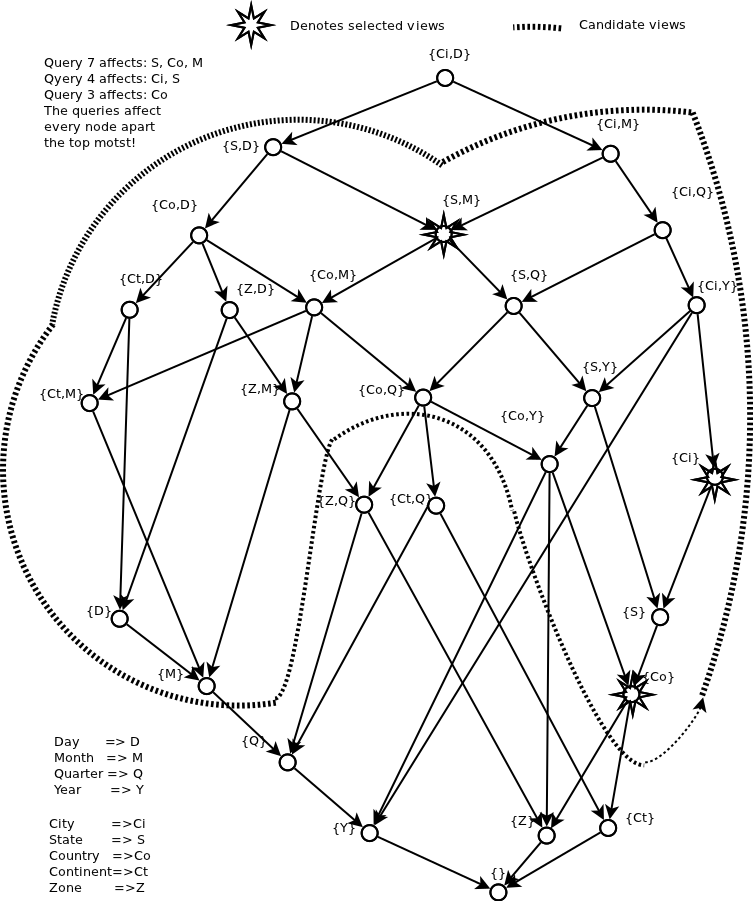
\includegraphics[scale=0.45]{lattice}
\caption{\label{fig:lattice}  Lattice}
\end{center}
\end{figure}

\subsection*{Summary} 
To conclude, this section about choosing and implementing materialised views we would like to stress some observation
which we have learned from our data.
\begin{itemize}
    \item For queries which {\bf aggregates heavily} and which has results a few rows, it {\bf always} pays of to use materialised views. In our example it is views $\{S,M\}$ and $\{Co\}$ see table above.
    \item All our Views including does not exceeds the smallest default block allocated by Oracle 
        \footnote{We used table $user\_extents$ to determine size of tables. See section $1)$ in Figure~\ref{s:details}.}
    \item Views speed up queries a lot, but if you do reuse the views in different queries,
    caching is probably easier alternative and works really well.
    \item Due to caching we have to "rename" our queries, 
    because we did not have sufficient privileges to turn caching off\footnote{
        See commands in section $2)$ in Figure~\ref{s:details}.}
    \item During design phase possibility of integrating views in star or snowflake schema should play role
    in deciding between snowflake and star schema.
    \item Oracle is capable of finding out itself that we used materialized views. 
    (We have to specify\footnote{See section $3)$ in Figure~\ref{s:details}.} it during creation.)
    On the other hand, it is not working very well, so basically you have to rewrite your queries.
\end{itemize}

\begin{figure}[!hbp]
\begin{center}
\begin{lstlisting}[language=sql] 
-- 1) determinig size of view or table
select segment_name table, sum(bytes)/(1024*1024) size_MB
from user_extents where segment_type='TABLE'
and segment_name = '&name' group by segment_name;

-- 2) disabling caching 1. method
ALTER SYSTEM FLUSH BUFFER_CACHE;
-- 2) disabling caching 2. method
ALTER TABLESPACE oplatek OFFLINE;

-- 3) enables rewriting the queries by using this views
create materialized view view_co 
    build immediate   --not relevant here
    enable query rewrite --this is important
    ...
\end{lstlisting}
\caption{\label{s:details}Technical details}
\end{center}
\end{figure}
